\documentclass[12pt]{article}

\usepackage[shortlabels]{enumitem}
\usepackage{graphicx}

\begin{document}

\title{Reporte de segunda tarea de Lenguajes de Programaci\'on}
\author{Diego Torres G.}
\date{\today}

\maketitle

\begin{enumerate}
\setcounter{enumi}{4}

		\item{La llamada (bundle '("a" "b" "c") 0) es un buen uso de bundle? ¿qu\'e produce? ¿por qu\'e?}\\\\
				De acuerdo a la definici\'on que usa los procedimientos "take" y "drop", usar $n = 0$, har\'ia que el procedimiento se cicle ya que en cada ocasi\'on se
				har\'ia una llamada recursiva a bundle con los mismos argumentos.\\

				Estar\'ias creando una lista infinita con todos sus elementos siendo listas vac\'ias.\\

				En la implementaci\'on que hay en esta tarea, bundle tira un error con $n = 0$.\\
\setcounter{enumi}{8}
\pagebreak

		\item{Dibuja un diagrama como el de la figura anterior pero para la lista '(11 9 2 18 12 14 4 1).}
				\begin{center}
						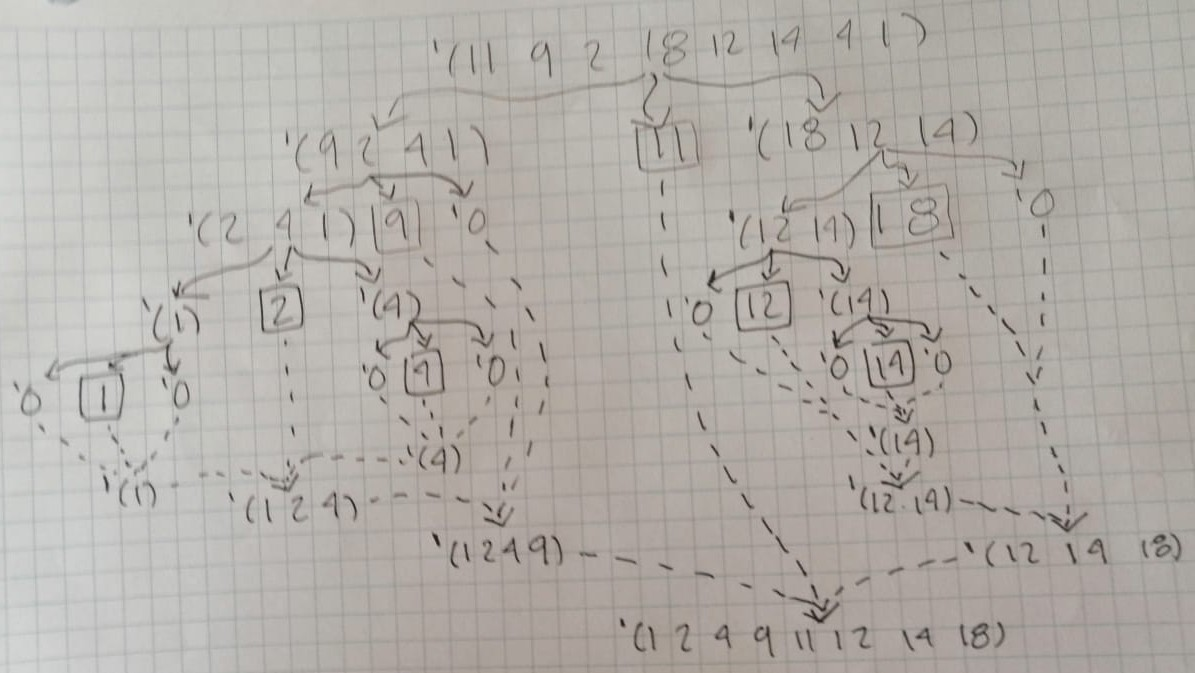
\includegraphics[scale=0.35]{quicksort_diagram.jpeg}
				\end{center}

\setcounter{enumi}{9}

		\item{Implementa los procedimientos smallers y largers.}\\
				De acuerdo a la definici\'on que se ped\'ia, cualquier elemento repetido se quedaba afuera.\\ Decid\'i cambiar el procedimiento largers por 
				larger-or-eq para admitir elementos repetidos.\\ En este caso y con esta implementación, en donde el pivote es el primer elemento, se mantiene la 
				estabilidad del algoritmo.

		\item{Si la entrada a quicksort contiene varias repeticiones de un número, va a regresar una lista estrictamente más corta que la entrada. 
				Responde el por qué y arregla el problema.}\\
				Como mecion\'e en el problema anterior, ya hab\'ia decidido modificar quicksort para aceptar repeticiones en la lista. Esto era porque
				para cada elecci\'on de pivote, se eliminaban las repeticiones de ese elemento al escoger solo los estrictamente mayores o menores.\\

\setcounter{enumi}{12}
		\item{Implementa una versión de quicksort que utilice isort si la longitud de la entrada está por debajo de un umbral. 
				Determina este umbral utilizando la función time, escribe el procedimiento que seguiste para encontrar este umbral.}\\

				Primero, mis supuestos; Tom\'e como si los n\'umeros generados por la funci\'on est\'andar 'random fueran variables independientes e identicamente
				distribuidas, adem\'as, que el tiempo medido por 'time-apply para cada ordenaci\'on no est\'a alterado por ning\'un factor externo de mi computadora
				o de cualquier otro tipo.\\ 
				Todo esto para decir que el tiempo promedio que tomar\'ia a un mismo algoritmo ordenar listas del mismo tama\~no generadas de la misma forma, 
				de acuerdo al teorema de Limite Central, es una variable aleatoria normal.\\

				Teniendo esto en cuenta, hice un procedimiento que mide el tiempo que toma a cada algoritmo ordenar una misma lista y regresa el tama\~no de entrada
				para el cu\'al quicksort es m\'as r\'apido que insertion sort.\\

				Para obtener un tama\~no de lista promedio, hice otro procedimiento que hace n experimentos y 
				calcula el valor esperado para esa muestra de n experimentos.\\

				Finalmente, saqu\'e el valor esperado con 100 experimentos y obtuve como resultado que quicksort es m\'as r\'apido para un tama\~no de entrada de 658
				elementos. Emp\'iricamente, observe que esta variable aleatoria no ten\'ia mucha desviaci\'on y me conform\'e con este n\'umero de experiementos.
				Adem\'as el tiempo que le tom\'o a mi computadora hacer este c\'alculo ya era bastante grande.\\

\setcounter{enumi}{16}
		\item{Modifica bundle para verificar que su entrada permita la terminación y que señale un error en caso contrario.}\\
				Bundle lanza un error en caso de que n sea negativo o cero. Esto nos asegura que en cada paso estamos resolviendo bundle con una lista
				m\'as peque\~na ya que estamos eliminando al menos un elemento en cada paso.

		\item{Considera la siguiente definición de smallers, uno de los procedimientos utilizados en quicksort, responde en qué puede fallar al 
				utilizar esta versión modificada en el procedimiento de ordenamiento.}\\
				
				Si la lista tiene elementos y el primero de ellos es mayor que el pivote, el procedimiento nunca termina porque se llama recursivamente a la
				funci\'on con los mismos argumentos.

		\item{Describe con tus propias palabras cómo funciona find-largest-divisor de gcd-structural. Responde por qué comienza desde (min n m).}\\
				Empieza con (min n m) porque todos los divisores de un n\'umero son menores o iguales que el n\'umero, dado que buscamos un divisor
				de n y m, el divisor no puede ser mayor que ninguno de los dos.\\

				Funciona checando si k es divisor de n y m y el siguiente caso es con el siguiente menor a k.\\

		\item{Describe con tus propias palabras cómo funciona find-largest-divisor de gcd-generative.}\\
				Se usa la propiedad de que (gcd l s) := (gcd s (remainder l s)). En cada caso (remainder l s) es menor que s por definici\'on. Reducimos los
				argumentos hasta llegar al caso base (= min 0), donde en el paso anterior el min, que ahora es el max,  era divisor del max anterior.\\

		\item{Utiliza la función time para determinar cuál de las dos implementaciones es más eficiente, escribiendo tu respuesta con los tiempos de ejecución 
				obtenidos con ambos procedimientos para valores “pequeños”, “medianos” y “grandes”. Justifica qué valores usaste en cada una de estas 
				mediciones y por qué los consideraste de ese “tamaño”.}\\

				De acuerdo a la funci\'on time, el procedimiento 'gcd-generative siempre es m\'as r\'apido, sin importar el tama\~no de las entradas. 
				Prob\'e entradas de dos digitos y la funci\'on a\'un no hac\'ia una medici\'on suficientemente precisa. Luego en los decenas de miles y 
				'gcd-generative fue m\'as r\'apido. Luego en las decenas de cientos de millones y 'gcd-generative termin\'o mientras que el estructural
				estaba tardando m\'as de lo que estaba dispuesto a esperar.\\

				Tambi\'en, se puede ver que 'gcd-structural tiene complejidad lineal en tiempo respecto a (min n m) y la de 'gcd-generative es logaritmica
				en tiempo respecto a (min n m).\\

		\item{Piensa y describe por qué no siempre es la mejor opción elegir el procedimiento más eficiente en tiempo de ejecución. Utiliza criterios que no 
				sean el de “eficiencia”.}\\

				\begin{itemize}
						\item{Legibilidad: Uno de los objetivos principales del c\'odigo es ser le\'ido por otras personas. Un pedazo de c\'odigo es mejor si
								se puede entender su modo de operar m\'as facilmente por un lector humano.}\\
						\item{Propiedades del algoritmo que implementa. Por ejemplo, hay ciertos algoritmos de ordenaci\'on que tienen la propiedad de estabilidad
								y, dependiendo del problema, puede ser m\'as importante que tiempo de ordenaci\'on.}\\
				\end{itemize}
				
\end{enumerate}


\end{document}
